\documentclass[a4paper, 12pt]{article}

\usepackage{amsmath, amsthm}

\usepackage{unicode-math}
\usepackage{xltxtra}
\usepackage{xgreek}
\setmainfont{Calibri}

\usepackage{fancyhdr}
\renewcommand{\footrulewidth}{0.4pt}% default is 0pt
\usepackage{lastpage}

\usepackage[a4paper, top=2.5cm, bottom=2.5cm, left=2.5cm, right=2.5cm, headheight=1cm, footskip=1.5cm]{geometry}
\usepackage[most]{tcolorbox}

\tcbuselibrary{listingsutf8}
\tcbset{
  theoremstyle/.style={
    colback=blue!5!white,
    colframe=blue!75!black,
    fonttitle=\bfseries,
    coltitle=black,
    colbacktitle=blue!10!white,
    enhanced,
    attach boxed title to top left={xshift=2mm,yshift=-2mm}
  },
}

\newcommand{\orismos}[1]{#1\index{\lowercase{#1}}}
\newtcolorbox[auto counter]{theorem}[2][]{%
  theoremstyle,
  before skip=20pt,
  title={Ορισμός~\thetcbcounter: \orismos{#2}}, #1
}

\renewenvironment{proof}[1][\textbf{Απάντηση}]{%
  \par\noindent\textbf{#1:} \rmfamily}{\qed\par}


\title{Ορισμοί Γ' Λυκείου}
\author{Κωνσταντίνος Λόλας}
\date{2025}

\usepackage{imakeidx}
\usepackage{hyperref}
\makeindex

\begin{document}

\pagestyle{fancy}
\fancyhead{} % clear all header fields
\fancyfoot{} % clear all footer fields
\fancyfoot[C]{\thepage\ από \pageref{LastPage}} % page number in the center
\fancyhead[L]{\textbf{Ορισμοί Γ' Λυκείου}} % left header
\fancyfoot[R]{\textbf{Κωνσταντίνος Λόλας}} % right footer

\maketitle

\begin{theorem}{Πραγματική Συνάρτηση}
  Έστω $Α$ ένα υποσύνολο του $\mathbb{R}$. Τι ονομάζουμε πραγματική συνάρτηση με πεδίο ορισμού το $Α$;
\end{theorem}
\begin{proof}
  Έστω $Α$ ένα υποσύνολο του $\mathbb{R}$. Ονομάζουμε πραγματική συνάρτηση με πεδίο ορισμού το $Α$ μια διαδικασία (κανόνα) $f$, με την οποία κάθε στοιχείο $x\in Α$ αντιστοιχίζεται σε ένα μόνο πραγματικό αριθμό $y$. Το $y$ ονομάζεται τιμή της $f$ στο $x$ και συμβολίζεται με $f(x)$.
\end{proof}

\begin{theorem}{Σύνολο Τιμών}
  Έστω $f$ μια συνάρτηση με πεδίο ορισμού το $A$. Πώς ορίζουμε το σύνολο τιμών της $f$;
\end{theorem}
\begin{proof}
  Το σύνολο των τιμών της $f$ ορίζεται ως το σύνολο
  $$f(A) = \{ f(x) | x \in A \}$$
\end{proof}

\begin{theorem}{Γραφική Παράσταση}
  Τι ονομάζουμε γραφική παράσταση μιας συνάρτησης $f$;
\end{theorem}
\begin{proof}
  Έστω $f$ μια συνάρτηση με πεδίο ορισμού $Α$ και $Oxy$ ένα σύστημα συντεταγμένων στο επίπεδο. Το σύνολο των σημείων $M(x, y)$ για τα οποία ισχύει $y = f(x)$, δηλαδή το σύνολο των σημείων $M(x, f(x))$, $x \in A$, λέγεται γραφική παράσταση της $f$ και συμβολίζεται συνήθως με $C_f$.
\end{proof}

\begin{theorem}{Ισότητα Συναρτήσεων}
  Πότε λέμε ότι δύο συναρτήσεις $f$ και $g$ είναι ίσες;
\end{theorem}
\begin{proof}
  Δύο συναρτήσεις $f$ και $g$ λέγονται ίσες όταν:
  \begin{itemize}
    \item έχουν το ίδιο πεδίο ορισμού $Α$ και
    \item για κάθε $x \in A$ ισχύει $f(x) = g(x)$.
  \end{itemize}
\end{proof}

\begin{theorem}{Πράξεις Συναρτήσεων}
  Έστω $f$ και $g$ δύο συναρτήσεις ορισμένες στα $Α$ και $Β$ αντίστοιχα. Πώς ορίζονται οι πράξεις άθροισμα, διαφορά, γινόμενο και πηλίκο των συναρτήσεων $f$ και $g$;
\end{theorem}
\begin{proof}
  Ορίζουμε ως άθροισμα $f + g$,  διαφορά $f - g$,  γινόμενο $fg$  και  πηλίκο $\dfrac{f}{g}$ δύο συναρτήσεων $f$, $g$ τις συναρτήσεις με τύπους:
  \begin{itemize}
    \item $(f + g)(x) = f(x) + g(x)$
    \item $(f - g)(x) = f(x) - g(x)$
    \item $(fg)(x) = f(x)g(x)$
    \item $\left(\dfrac{f}{g}\right)(x) = \dfrac{f(x)}{g(x)}$.
  \end{itemize}
  Το πεδίο ορισμού των $f+g$, $f-g$, $fg$ είναι η τομή $A \cap B$ των πεδίων ορισμού των συναρτήσεων $f$ και $g$, ενώ το πεδίο ορισμού της $\frac{f}{g}$ είναι το $A \cap B$ εξαιρουμένων των τιμών του $x$ που μηδενίζουν τον παρανομαστή $g$. δηλαδή
  $$ \{ x|x\in A \cap B, g(x) \neq 0 \}$$
\end{proof}

\begin{theorem}{Σύνθεση Συναρτήσεων}
  Έστω $f$ και $g$ δύο συναρτήσεις ορισμένες στα $A$ και $B$ αντίστοιχα. Πώς ορίζεται η σύνθεση των συναρτήσεων $f$ και $g$;
\end{theorem}
\begin{proof}
  Αν $f$, $g$ είναι δύο συναρτήσεις με πεδίο ορισμού $Α$, $Β$ αντιστοίχως, τότε ονομάζουμε σύνθεση της $f$ με την $g$, και τη συμβολίζουμε με $g\circ f$, τη συνάρτηση με τύπο
  $$(g\circ f)(x) = g(f(x))$$
  \begin{center}
    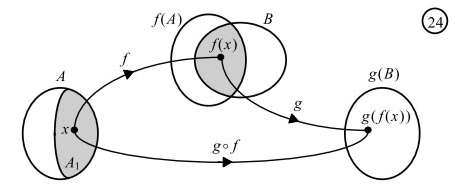
\includegraphics[width=0.5\textwidth]{images/1.2 Σύνθεση}
  \end{center}
  Το πεδίο ορισμού της $g\circ f$ αποτελείται από όλα τα στοιχεία $x$ του πεδίου ορισμού της $f$ για τα οποία το $f(x)$ ανήκει στο πεδίο ορισμού της $g$. Δηλαδή είναι το σύνολο
  $A_1 = \{ x \in A   |   f(x) \in Β\}$
\end{proof}

\begin{theorem}{Γνησίως Αύξουσα Συνάρτηση}
  Πότε μια συνάρτηση $f$ λέγεται γνησίως αύξουσα σε ένα διάστημα $Δ$;
\end{theorem}
\begin{proof}
  Μια συνάρτηση $f$ λέγεται γνησίως αύξουσα σε ένα διάστημα $Δ$ του πεδίου ορισμού της, όταν για οποιαδήποτε $x_1$, $x_2 \in Δ$ με $x_1 < x_2$ ισχύει $f(x_1) < f(x_2)$.
\end{proof}

\begin{theorem}{Γνησίως Φθίνουσα Συνάρτηση}
  Πότε μια συνάρτηση $f$ λέγεται γνησίως φθίνουσα σε ένα διάστημα $Δ$;
\end{theorem}
\begin{proof}
  Μια συνάρτηση $f$ λέγεται γνησίως φθίνουσα σε ένα διάστημα $Δ$ του πεδίου ορισμού της, όταν για οποιαδήποτε $x_1$, $x_2 \in Δ$ με $x_1 < x_2$ ισχύει $f(x_1) > f(x_2)$.
\end{proof}

\begin{theorem}{Αύξουσα Συνάρτηση}
  Πότε μια συνάρτηση $f$ λέγεται αύξουσα σε ένα διάστημα $Δ$;
\end{theorem}
\begin{proof}
  Μια συνάρτηση $f$ λέγεται αύξουσα σε ένα διάστημα $Δ$ αν για κάθε $x_1$, $x_2 \in Δ$ με $x_1 < x_2$ ισχύει $f(x_1) \leq f(x_2)$.
\end{proof}

\begin{theorem}{Φθίνουσα Συνάρτηση}
  Πότε μια συνάρτηση $f$ λέγεται φθίνουσα σε ένα διάστημα $Δ$;
\end{theorem}
\begin{proof}
  Μια συνάρτηση $f$ λέγεται φθίνουσα σε ένα διάστημα $Δ$ αν για κάθε $x_1$, $x_2 \in Δ$ με $x_1 < x_2$ ισχύει $f(x_1) \geq f(x_2)$.
\end{proof}

\begin{theorem}{Γνησίως Μονότονη Συνάρτηση}
  Πότε μια συνάρτηση $f$ λέγεται γνησίως μονότονη σε ένα διάστημα $Δ$;
\end{theorem}
\begin{proof}
  Μια συνάρτηση $f$ λέγεται γνησίως μονότονη σε ένα διάστημα $Δ$ αν είναι γνησίως αύξουσα ή γνησίως φθίνουσα σε αυτό.
\end{proof}

\begin{theorem}{Μέγιστο}
  Πότε μια συνάρτηση $f$ με πεδίο ορισμού το $A$ θα λέμε ότι έχει μέγιστο στο $x_0$;
\end{theorem}
\begin{proof}
  Έστω $f$ μια συνάρτηση με πεδίο ορισμού το $A$. Θα λέμε ότι η $f$ παρουσιάζει στο $x_0\in Α$ μέγιστο το $f(x_0)$ αν ισχύει:
  $$f(x_0) \geq f(x) \quad \text{ για κάθε } x \in A$$
\end{proof}

\begin{theorem}{Ελάχιστο}
  Πότε μια συνάρτηση $f$ με πεδίο ορισμού το $A$ θα λέμε ότι έχει ελάχιστο στο $x_0$;
\end{theorem}
\begin{proof}
  Έστω $f$ μια συνάρτηση με πεδίο ορισμού το $A$. Θα λέμε ότι η $f$ παρουσιάζει στο $x_0\in Α$ ελάχιστο το $f(x_0)$ αν ισχύει:
  $$f(x_0) \leq f(x) \quad \text{ για κάθε } x \in A$$
\end{proof}

\begin{theorem}{Ακρότατα}
  Τι ονομάζουμε ακρότατα μιας συνάρτησης $f$;
\end{theorem}
\begin{proof}
  Το μέγιστο και το ελάχιστο μιας συνάρτησης $f$ λέγονται ολικά ακρότατα της $f$.
\end{proof}

\begin{theorem}{1-1}
  Πότε μια συνάρτηση $f$ λέγεται 1-1;
\end{theorem}
\begin{proof}
  Μια συνάρτηση $f$ λέγεται 1-1 αν για κάθε $x_1$, $x_2 \in A$ με $x_1 \neq x_2$ ισχύει $f(x_1) \neq f(x_2)$.
\end{proof}

\begin{theorem}{Αντίστροφη Συνάρτηση}
  Πώς ορίζεται η αντίστροφη συνάρτηση μιας $f$;
\end{theorem}
\begin{proof}
  Έστω μια συνάρτηση $f : A \to \mathbb{R}$. Αν υποθέσουμε ότι αυτή είναι 1–1, τότε για κάθε στοιχείο $y$ του συνόλου τιμών, $f(A)$, της $f$ υπάρχει μοναδικό στοιχείο $x$ του πεδίου ορισμού της $Α$ για το οποίο ισχύει $f(x) = y$. Επομένως ορίζεται μια συνάρτηση
  $g : f ( A) \to \mathbb{R}$ με την οποία κάθε $y \in f ( A)$ αντιστοιχίζεται στο μοναδικό $x \in A$ για το οποίο ισχύει $f(x) = y$.
\end{proof}

\begin{theorem}{Κριτήριο Παρεμβολής}
  Να διατυπώσετε το κριτήριο παρεμβολής
\end{theorem}
\begin{proof}
  Έστω οι συναρτήσεις $f$, $g$, $h$. Αν
  \begin{itemize}
    \item $h(x) \leq f(x) \leq g(x)$ για κάθε $x$ κοντά στο $x_0$ και
    \item $\lim_{x \to x_0} h(x) = \lim_{x \to x_0} g(x) = λ$,
  \end{itemize}
  τότε
  $$\lim_{x \to x_0} f(x) = λ$$
\end{proof}

\begin{theorem}{Ακολουθία}
  Να δώσετε τον ορισμό της ακολουθίας.
\end{theorem}
\begin{proof}
  Ακολουθία ονομάζεται κάθε πραγματική συνάρτηση $α : \mathbb{N}^* \to \mathbb{R}$.
\end{proof}

\begin{theorem}{Συνέχεια σε σημείο}
  Να δώσετε τον ορισμό της συνέχειας σε σημείο $x_0$.
\end{theorem}
\begin{proof}
  Έστω μια συνάρτηση $f$ και $x_0$ ένα σημείο του πεδίου ορισμού της. Θα λέμε ότι η $f$ είναι συνεχής στο $x_0$, όταν
  $$\lim_{x \to x_0} f(x) = f(x_0)$$
\end{proof}

\begin{theorem}{Συνεχής Συνάρτηση}
  Πότε λέμε ότι μια συνάρτηση $f$ είναι συνεχής;
\end{theorem}
\begin{proof}
  Μια συνάρτηση $f$ λέγεται συνεχής αν είναι συνεχής σε κάθε σημείο του πεδίου ορισμού της.
\end{proof}

\begin{theorem}{Συνέχεια σε ανοιχτό διάστημα}
  Πότε λέμε ότι μια συνάρτηση $f$ είναι συνεχής σε ένα ανοικτό διάστημα  $(α, β)$;
\end{theorem}
\begin{proof}
  Μια συνάρτηση $f$ θα λέμε ότι είναι συνεχής σε ένα ανοικτό διάστημα $(α, β)$, όταν είναι συνεχής σε κάθε σημείο του $(α, β)$
\end{proof}

\begin{theorem}{Συνέχεια σε κλειστό διάστημα}
  Πότε λέμε ότι μια συνάρτηση $f$ είναι συνεχής σε ένα κλειστό διάστημα  $[α, β]$;
\end{theorem}
\begin{proof}
  Μια συνάρτηση $f$ θα λέμε ότι είναι συνεχής σε ένα κλειστό διάστημα $[α, β]$, όταν είναι συνεχής στο ανοιχτό $(α, β)$ και επιπλέον
  \begin{itemize}
    \item $\lim_{x \to α^+} f(x) = f(α)$
    \item $\lim_{x \to β^-} f(x) = f(β)$
  \end{itemize}
\end{proof}

\begin{theorem}{Θεώρημα Bolzano}
  Να διατυπώσετε το θεώρημα Bolzano.
\end{theorem}
\begin{proof}
  Έστω μια συνάρτηση $f$, ορισμένη σε ένα κλειστό διάστημα $[α, β]$. Αν:
  \begin{itemize}
    \item η $f$ είναι συνεχής στο $[α, β]$ και
    \item $f(α)\cdot f(β) < 0$
  \end{itemize}
  τότε υπάρχει ένα, τουλάχιστον, $x_0 \in (α,β )$ τέτοιο, ώστε $f(x_0) = 0$.
  Δηλαδή, υπάρχει μια, τουλάχιστον, ρίζα της εξίσωσης $f(x) = 0$ στο ανοικτό διάστημα $(α, β)$.
\end{proof}

\begin{theorem}{Γεωμετρική ερμηνεία θ. Bolzano }
  Να δώσετε τη γεωμετρική ερμηνεία του θεωρήματος Bolzano.
\end{theorem}
\begin{proof}
  Στο διπλανό σχήμα έχουμε τη γραφική παράσταση μιας συνεχούς συνάρτησης $f$ στο $[α, β]$. Επειδή τα σημεία $Α(α, f(α))$ και $Β(β, f(β))$ βρίσκονται εκατέρωθεν του άξονα $x′x$, η γραφική παράσταση της $f$ τέμνει τον άξονα σε ένα τουλάχιστον σημείο.
  \begin{center}
    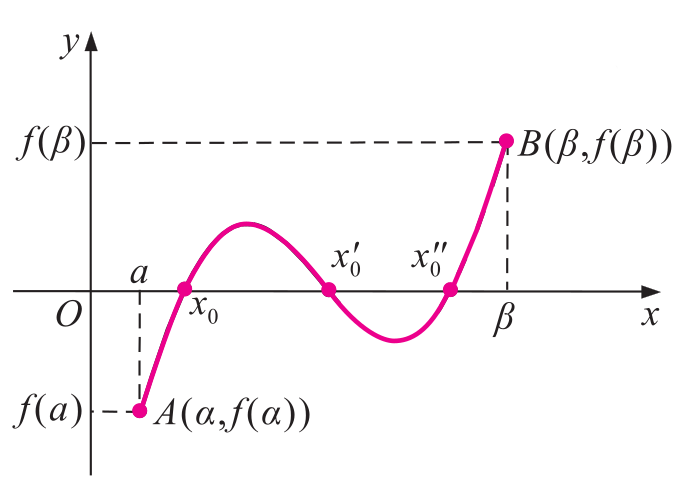
\includegraphics[width=0.5\textwidth]{images/geoBolzano}
  \end{center}
\end{proof}

\begin{theorem}{Θεώρημα Ενδιάμεσων Τιμών}
  Να διατυπώσετε το θεώρημα Ενδιάμεσων Τιμών.
\end{theorem}
\begin{proof}
  Έστω μια συνάρτηση $f$, η οποία είναι ορισμένη σε ένα κλειστό διάστημα $[α, β]$. Αν:
  \begin{itemize}
    \item η $f$ είναι συνεχής στο $[α, β]$ και
    \item $f(α) \neq f(β)$
  \end{itemize}
  τότε, για κάθε αριθμό $η$ μεταξύ των $f(α)$ και $f(β)$ υπάρχει ένας, τουλάχιστον
  $x_0 \in (α , β )$ τέτοιος, ώστε
  $f(x_0) = η$
\end{proof}

\begin{theorem}{Γεωμετρική ερμηνεία Θ.Ε.Τ.}
  Να δώσετε τη γεωμετρική ερμηνεία του θεώρηματος Ενδιάμεσων Τιμών.
\end{theorem}
\begin{proof}
  Στο διπλανό σχήμα έχουμε τη γραφική παράσταση μιας συνεχούς συνάρτησης $f$ στο $[α, β]$. Επειδή η $f$ είναι συνεχής στο $[α, β]$, η γραφική της παράσταση είναι μια συνεχή καμπύλη. Αν $η$ είναι ένας αριθμός μεταξύ των $f(α)$ και $f(β)$, τότε η γραφική παράσταση της $f$ τέμνει την οριζόντια ευθεία $y = η$ σε ένα τουλάχιστον σημείο.
  \begin{center}
    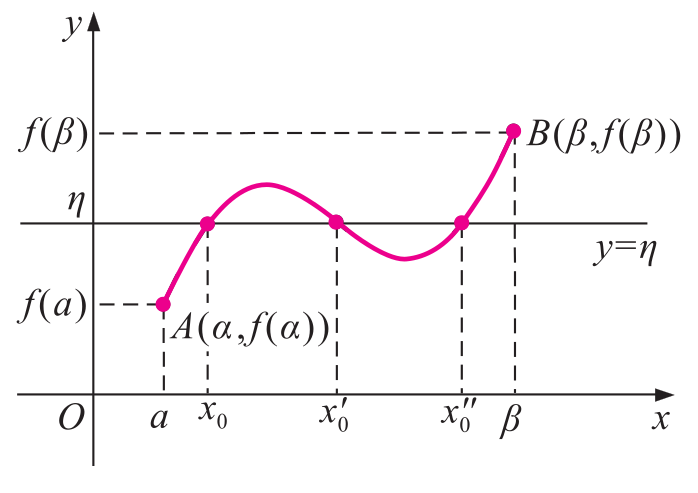
\includegraphics[width=0.5\textwidth]{images/geoBolzano2}
  \end{center}
\end{proof}

\begin{theorem}{Θεώρημα Μέγιστης και Ελάχιστης τιμής}
  Να διατυπώσετε το θεώρημα μέγιστης και ελάχιστης τιμής.
\end{theorem}
\begin{proof}
  Αν $f$ είναι συνεχής συνάρτηση στο $[α, β]$, τότε η $f$ παίρνει στο $[α, β]$ μια μέγιστη τιμή $Μ$ και μια ελάχιστη τιμή $m$.
\end{proof}

\begin{theorem}{Εφαπτομένη}
  Πώς ορίζεται η εφαπτομένη μιας συνάρτησης $f$ στο σημείο της $(x_0, f(x_0))$;
\end{theorem}
\begin{proof}
  Έστω $f$ μια συνάρτηση και $Α(x_0, f( x_0))$ ένα σημείο της $C_f$. Αν υπάρχει το
  $$\lim_{x \to x_0} \dfrac{f(x) - f(x_0)}{x - x_0}$$
  και είναι ένας πραγματικός αριθμός $λ$, τότε ορίζουμε ως εφαπτομένη της $C_f$ στο σημείο της $A$, την ευθεία $ε$ που διέρχεται από το $A$ και έχει συντελεστή διεύθυνσης $λ$.
\end{proof}

\begin{theorem}{Παραγωγισιμότητα σε σημείο}
  Πότε λέμε ότι μια συνάρτηση $f$ είναι παραγωγίσιμη στο $x_0$;
\end{theorem}
\begin{proof}
  Μια συνάρτηση $f$ λέμε ότι είναι παραγωγίσιμη σ’ ένα σημείο $x_0$ του πεδίου ορισμού της, αν υπάρχει το
  $$\lim_{x \to x_0} \dfrac{f(x) - f(x_0)}{x - x_0}$$
  και είναι πραγματικός αριθμός. Το όριο αυτό ονομάζεται παράγωγος της $f$ στο $x_0$ και συμβολίζεται με $f'(x_0)$.
  Δηλαδή:
  $$f'(x_0) = \lim_{x \to x_0} \dfrac{f(x) - f(x_0)}{x - x_0}$$
\end{proof}

\begin{theorem}{Παραγωγίσιμη συνάρτηση}
  Πότε λέμε ότι μια συνάρτηση $f$ είναι παραγωγίσιμη στο $A\subseteq \mathbb{R}$;
\end{theorem}
\begin{proof}
  Μια συνάρτηση $f$ λέμε ότι είναι παραγωγίσιμη στο $A\subseteq \mathbb{R}$, αν είναι παραγωγίσιμη σε κάθε σημείο $x\in A$.
\end{proof}

\begin{theorem}{Παραγωγισιμότητα σε ανοικτό διάστημα}
  Πότε λέμε ότι μια συνάρτηση $f$ είναι παραγωγίσιμη σε ένα ανοικτό διάστημα $(α,β)$ του πεδίου ορισμού της;
\end{theorem}
\begin{proof}
  Μια συνάρτηση $f$ λέμε ότι είναι παραγωγίσιμη σε ένα ανοικτό διάστημα $(α, β)$ του πεδίου ορισμού της, όταν είναι παραγωγίσιμη σε κάθε σημείο $x_0 \in (α , β )$.
\end{proof}

\begin{theorem}{Παραγωγισιμότητα σε κλειστό διάστημα}
  Πότε λέμε ότι μια συνάρτηση $f$ είναι παραγωγίσιμη σε ένα κλειστό διάστημα $[α, β]$ του πεδίου ορισμού της;
\end{theorem}
\begin{proof}
  Μια συνάρτηση $f$ λέμε ότι είναι παραγωγίσιμη σε ένα κλειστό διάστημα $[α, β]$ του πεδίου ορισμού της, όταν είναι παραγωγίσιμη σε κάθε σημείο $x_0 \in (α , β )$ και επιπλέον
  $$\lim_{x \to α^+} f'(x) \in \mathbb{R} \text{ και } \lim_{x \to β^-} f'(x) \in \mathbb{R}$$
\end{proof}

\begin{theorem}{Παράγωγος συνάρτηση}
  Πώς ορίζεται η παράγωγος συνάρτηση μιας $f$;
\end{theorem}
\begin{proof}
  Έστω $f$ μια συνάρτηση με πεδίο ορισμού $A$ και $A_1$ το σύνολο των σημείων του $A$ στα
  οποία αυτή είναι παραγωγίσιμη. Αντιστοιχίζοντας κάθε $x \in A_1$ στο $f'(x)$, ορίζουμε τη συνάρτηση
  $$f' : A_1 \to \mathbb{R}$$
  $$x \mapsto f'(x)$$
  η οποία ονομάζεται πρώτη παράγωγος της $f$ ή απλά παράγωγος της $f$.
\end{proof}

\begin{theorem}{Ρυθμός μεταβολής}
  Πώς ορίζεται ο ρυθμός μεταβολής του $y$ ως προς το $x$ στο σημείο $x_0$;
\end{theorem}
\begin{proof}
  Αν δύο μεταβλητά μεγέθη $x$, $y$ συνδέονται με τη σχέση $y = f ( x)$, όταν $f$ είναι μια συνάρτηση παραγωγίσιμη στο $x_0$, τότε ονομάζουμε ρυθμό μεταβολής του $y$ ως προς το $x$ στο σημείο $x_0$ την παράγωγο $f'(x_0)$.
\end{proof}

\begin{theorem}{Θεώρημα Rolle}
  Να διατυπώσετε το θεώρημα Rolle.
\end{theorem}
\begin{proof}
  Αν μια συνάρτηση $f$ είναι:
  \begin{itemize}
    \item συνεχής στο κλειστό διάστημα $[α, β]$
    \item παραγωγίσιμη στο ανοικτό διάστημα $(α, β)$ και
    \item $f(α) = f(β)$
  \end{itemize}
  τότε υπάρχει ένα, τουλάχιστον, $ξ \in (α , β )$ τέτοιο, ώστε:
  $$f ′(ξ) = 0$$
\end{proof}

\begin{theorem}{Γεωμετρική ερμηνεία Θ. Rolle}
  Να δώσετε τη γεωμετρική ερμηνεία του θεωρήματος Rolle.
\end{theorem}
\begin{proof}
  Στο διπλανό σχήμα έχουμε τη γραφική παράσταση μιας συνεχούς συνάρτησης $f$ στο $[α, β]$. Επειδή η $f$ είναι συνεχής στο $[α, β]$, η γραφική της παράσταση είναι μια συνεχή καμπύλη. Επίσης, επειδή $f(α) = f(β)$, υπάρχει τουλάχιστον ένα σημείο $ξ$ της $C_f$ στο οποίο η εφαπτομένη είναι παράλληλη στον άξονα $x′x$. Δηλαδή, η $f ′(ξ) = 0$.
  \begin{center}
    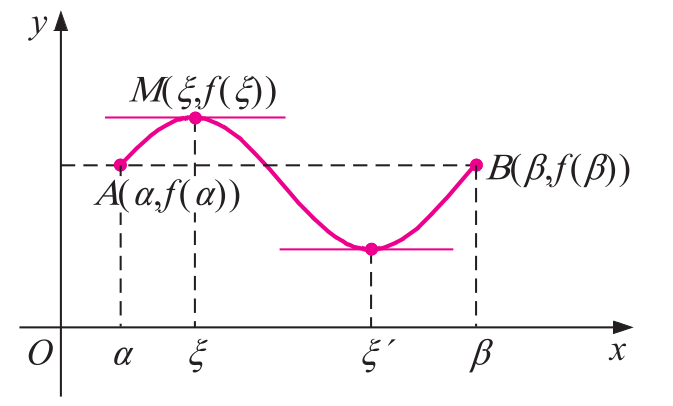
\includegraphics[width=0.5\textwidth]{images/geoRolle}
  \end{center}
\end{proof}

\begin{theorem}{Θεώρημα Μέσης Τιμής}
  Να διατυπώσετε το θεώρημα μέσης τιμής.
\end{theorem}
\begin{proof}
  Αν μια συνάρτηση $f$ είναι:
  \begin{itemize}
    \item συνεχής στο κλειστό διάστημα $[α, β]$
    \item παραγωγίσιμη στο ανοικτό διάστημα $(α, β)$
  \end{itemize}
  τότε υπάρχει ένα, τουλάχιστον, $ξ \in (α , β )$ τέτοιο, ώστε:
  $$f ′(ξ) = \dfrac{f(β) - f(α)}{β - α}$$
\end{proof}

\begin{theorem}{Γεωμετρική ερμηνεία Θ.Μ.Τ.}
  Να δώσετε τη γεωμετρική ερμηνεία του θεωρήματος μέσης τιμής.
\end{theorem}
\begin{proof}
  Στο διπλανό σχήμα έχουμε τη γραφική παράσταση μιας συνεχούς συνάρτησης $f$ στο $[α, β]$. Επειδή η $f$ είναι συνεχής στο $[α, β]$, η γραφική της παράσταση είναι μια συνεχή καμπύλη. Υπάρχει τουλάχιστον ένα σημείο $ξ$ της $C_f$ στο οποίο η εφαπτομένη είναι παράλληλη στην εφαπτομένη της ευθείας που ενώνει τα σημεία $A(α, f(α))$ και $B(β, f(β))$.
  \begin{center}
    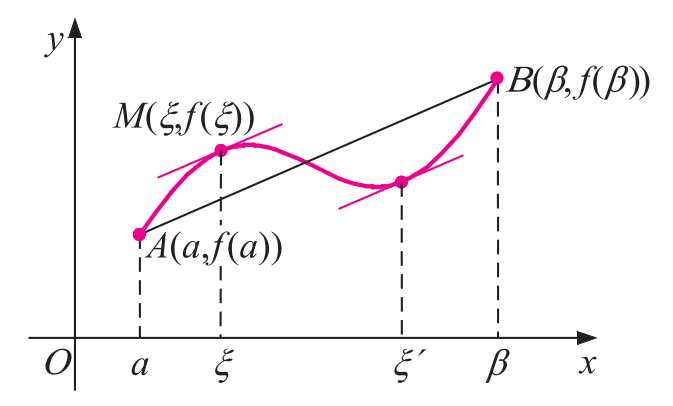
\includegraphics[width=0.5\textwidth]{images/geoTMT}
  \end{center}
\end{proof}

\begin{theorem}{Τοπικό μέγιστο}
  Πώς ορίζεται το τοπικό μέγιστο μιας συνάρτησης $f$ στο $x_0$;
\end{theorem}
\begin{proof}
  Μια συνάρτηση $f$, με πεδίο ορισμού $A$, θα λέμε ότι παρουσιάζει στο $x_0 \in A$ τοπικό μέγιστο, όταν υπάρχει $δ > 0$, τέτοιο ώστε
  $$f ( x) \leq f ( x_0 )$$
  για κάθε $x \in A \cap ( x_0 − δ , x_0 + δ )$.
  Το $x_0$ λέγεται θέση ή σημείο τοπικού μεγίστου, ενώ το $f(x_0)$ το τοπικό μέγιστο της $f$.
\end{proof}

\begin{theorem}{Τοπικό ελάχιστο}
  Πώς ορίζεται το τοπικό ελάχιστο μιας συνάρτησης $f$ στο $x_0$;
\end{theorem}
\begin{proof}
  Μια συνάρτηση $f$, με πεδίο ορισμού $A$, θα λέμε ότι παρουσιάζει στο $x_0 \in A$ τοπικό ελάχιστο, όταν υπάρχει $δ > 0$, τέτοιο ώστε
  $$f ( x) \geq f ( x_0 )$$
  για κάθε $x \in A \cap ( x_0 − δ , x_0 + δ )$.
  Το $x_0$ λέγεται θέση ή σημείο τοπικού ελαχίστου, ενώ το $f(x_0)$ το τοπικό ελάχιστο της $f$.
\end{proof}

\begin{theorem}{Θεώρημα Fermat}
  Να διατυπώσετε το θεώρημα Fermat.
\end{theorem}
\begin{proof}
  Έστω μια συνάρτηση $f$ ορισμένη σ’ ένα διάστημα $Δ$ και $x_0$ ένα εσωτερικό σημείο του $Δ$. Αν η $f$ παρουσιάζει τοπικό μέγιστο ή τοπικό ελάχιστο στο $x_0$ και είναι παραγωγίσιμη στο σημείο αυτό, τότε:
  $$f ′(x_0) = 0$$
\end{proof}

\begin{theorem}{Πιθανές θέσεις τοπικών ακροτάτων}
  Έστω μια συνάρτηση $f$ ορισμένη σε ένα διάστημα $Δ$. Ποιες είναι οι πιθανές θέσεις τοπικών ακροτάτων της $f$ στο $Δ$;
\end{theorem}
\begin{proof}
  Οι πιθανές θέσεις τοπικών ακροτάτων της $f$ στο διάστημα $Δ$ είναι:
  \begin{itemize}
    \item Τα εσωτερικά σημεία του $Δ$ στα οποία η παράγωγος της $f$ μηδενίζεται.
    \item Τα εσωτερικά σημεία του $Δ$ στα οποία η $f$ δεν παραγωγίζεται.
    \item Τα άκρα του $Δ$ (αν ανήκουν στο πεδίο ορισμού της).
  \end{itemize}
\end{proof}

\begin{theorem}{Κρίσιμα σημεία}
  Πώς ορίζονται τα κρίσιμα σημεία μιας συνάρτησης $f$;
\end{theorem}
\begin{proof}
  Τα εσωτερικά σημεία του $Δ$ στα οποία η $f$ δεν παραγωγίζεται ή η παράγωγός της είναι ίση με το μηδέν, λέγονται κρίσιμα σημεία της $f$ στο διάστημα $Δ$.
\end{proof}

\begin{theorem}{Κυρτή συνάρτηση}
  Πώς ορίζεται μια κυρτή συνάρτηση $f$ στο $Δ$;
\end{theorem}
\begin{proof}
  Έστω μία συνάρτηση $f$ συνεχής σ' ένα διάστημα $Δ$ και παραγωγίσιμη στο εσωτερικό του $Δ$. Θα λέμε ότι η συνάρτηση $f$ στρέφει τα κοίλα προς τα κάτω ή είναι κυρτή στο $Δ$, αν η $f '$ είναι γνησίως φθίνουσα στο εσωτερικό του $Δ$.
\end{proof}

\begin{theorem}{Κοίλη συνάρτηση}
  Πώς ορίζεται μια κοίλη συνάρτηση $f$ στο $Δ$;
\end{theorem}
\begin{proof}
  Έστω μία συνάρτηση $f$ συνεχής σ' ένα διάστημα $Δ$ και παραγωγίσιμη στο εσωτερικό του $Δ$. Θα λέμε ότι η συνάρτηση $f$ στρέφει τα κοίλα προς τα πάνω ή είναι κοίλη στο $Δ$, αν η $f '$ είναι γνησίως αύξουσα στο εσωτερικό του $Δ$.
\end{proof}

\begin{theorem}{Σημείο καμπής}
  Πώς ορίζεται το σημείο καμπής μιας συνάρτησης $f$ στο $x_0$;
\end{theorem}
\begin{proof}
  Έστω μια συνάρτηση $f$ παραγωγίσιμη σ’ ένα διάστημα $(α, β)$, με εξαίρεση ίσως ένα
  σημείο του $x_0$. Αν
  \begin{itemize}
    \item η $f$ είναι κυρτή στο $(α, x_0)$ και κοίλη στο $(x_0, β)$, ή αντιστρόφως, και
    \item η $C_f$ έχει εφαπτομένη στο σημείο $A(x_0, f(x_0))$,
  \end{itemize}
  τότε το σημείο $A(x_0, f(x_0))$ ονομάζεται σημείο καμπής της γραφικής παράστασης
  της $f$.
\end{proof}

\begin{theorem}{Πιθανές θέσεις σημείων καμπής}
  Ποιες είναι οι πιθανές θέσεις σημείων καμπής μιας συνάρτησης $f$;
\end{theorem}
\begin{proof}
  Οι πιθανές θέσεις σημείων καμπής μιας συνάρτησης $f$ σ’ ένα διάστημα $Δ$ είναι:
  \begin{itemize}
    \item Τα εσωτερικά σημεία του $Δ$ στα οποία η $f ''$ μηδενίζεται.
    \item Τα εσωτερικά σημεία του $Δ$ στα οποία δεν υπάρχει η $f ''$.
  \end{itemize}
\end{proof}

\begin{theorem}{Κατακόρυφη ασύμπτωτη}
  Πώς ορίζεται η κατακόρυφη ασύμπτωτη μιας συνάρτησης $f$;
\end{theorem}
\begin{proof}
  Αν ένα τουλάχιστον από τα όρια
  $$\lim_{x \to x_0} f ( x) = +\infty \text{ ή } \lim_{x \to x_0} f ( x) = −\infty$$
  τότε η ευθεία $x = x_0$ λέγεται κατακόρυφη ασύμπτωτη της γραφικής παράστασης της $f$.
\end{proof}

\begin{theorem}{Οριζόντια ασύμπτωτη}
  Πώς ορίζεται η οριζόντια ασύμπτωτη μιας συνάρτησης $f$;
\end{theorem}
\begin{proof}
  Αν $\lim_{x \to +\infty} f ( x) = λ$ (αντιστοίχως $\lim_{x \to -\infty} f ( x) = λ$), τότε η ευθεία $y = λ$ λέγεται οριζόντια ασύμπτωτη της γραφικής παράστασης της $f$ στο $+\infty$ (αντιστοίχως στο $−\infty$).
\end{proof}

\begin{theorem}{Ασύμπτωτη}
  Πώς ορίζεται η ασύμπτωτη μιας συνάρτησης $f$;
\end{theorem}
\begin{proof}
  Η ευθεία $y = λx + β$ λέγεται ασύμπτωτη της γραφικής παράστασης της $f$ στο $+\infty$ (αντιστοίχως στο $−\infty$), αν
  $$\lim_{x \to +\infty} [ f ( x) − (λ x + β )] = 0$$
  (αντιστοίχως $\lim_{x \to -\infty} [ f ( x) − (λ x + β )] = 0$).
\end{proof}

\begin{theorem}{Κανόνας de L' Hospital}
  Να διατυπώσετε το κανόνα de L' Hospital.
\end{theorem}
\begin{proof}
  Αν $\lim_{x \to x_0} f ( x) = 0$, $\lim_{x \to x_0} g ( x) = 0$, $x_0 \in \mathbb{R} \cup \{−\infty, + \infty\}$ και υπάρχει το
  $$\lim_{x \to x_0} \dfrac{f'( x)}{g' ( x)}$$
  (περασμένο ή άπειρο), τότε:
  $$\lim_{x \to x_0} \dfrac{f ( x)}{g ( x)} = \lim_{x \to x_0} \dfrac{f' ( x)}{g' ( x)}$$
\end{proof}

\begin{theorem}{Αρχική συνάρτηση}
  Πώς ορίζεται η αρχική συνάρτηση μιας $f$;
\end{theorem}
\begin{proof}
  Έστω $f$ μια συνάρτηση ορισμένη σε ένα διάστημα $Δ$. Αρχική συνάρτηση ή παράγωγος της $f$ στο $Δ$ ονομάζεται κάθε συνάρτηση $F$ που είναι παραγωγίσιμη στο $Δ$ και ισχύει
  $$F ′ (x) = f(x), \text{ για κάθε } x \in Δ$$
\end{proof}

\begin{theorem}{Ορισμένο ολοκλήρωμα}
  Πώς ορίζεται το ορισμένο ολοκλήρωμα μιας $f$ στο $[α, β]$;
\end{theorem}
\begin{proof}
  Έστω $f$ μια συνάρτηση ορισμένη στο $[α, β]$. Το ορισμένο ολοκλήρωμα της $f$ στο $[α, β]$ ορίζεται ως το όριο
  $$\lim_{n \to \infty} \sum_{i=1}^{n} f ( ξ_i ) Δx$$
  όπου $Δx = \dfrac{b - a}{n}$ και $ξ_i \in [x_{i-1}, x_i]$, έτσι
  $$\int_{α}^{β} f ( x) dx = \lim_{n \to \infty} \sum_{i=1}^{n} f ( ξ_i ) Δx$$
\end{proof}

\begin{theorem}{Θεμελιώδες θεώρημα του ολοκληρωτικού λογισμού}
  Να διατυπώσετε το θεμελιώδες θεώρημα του ολοκληρωτικού λογισμού.
\end{theorem}
\begin{proof}
  Έστω f μια συνεχής συνάρτηση σ’ ένα διάστημα [α, β]. Αν G είναι μια παράγουσα
  της f στο [α, β], τότε
  $$\int_{α}^{β} f (x) dx = G(β) − G(α)$$
\end{proof}

\printindex

\end{document}